\chapter[Resultados: clasificación y detección de melanoma]{Resultados: clasificación diagnóstica y detección de melanoma}
\label{cp:res_clasif}
% Extensión estimada: 20--25 páginas.
% Fuentes: sección "Clasificación diagnóstica" del documento de experimentación, con los números del split
% disjunto por lesión (Codigo/outputs/results/lesion_split_report.json, cerrado el 2026-09-15 con las
% semillas 42/43/44).
%
% Feedback del tutor (14/09/2026): la sección de cierre se llama "Discusión" en lugar de "Síntesis del
% capítulo". La discusión transversal, que cruza este capítulo con el de generación, queda en el
% Capítulo~\ref{cp:discusion}.

% Introducción redactada el 24/10/2026 (ficha 00-capitulo.md): por contenido, sin «responde la PI1», con las
% convenciones que valen para todas las cifras del capítulo.

Este capítulo presenta los resultados de la clasificación de lesiones de piel y de la detección de melanoma. Primero
se comparan las cuatro arquitecturas supervisadas y se analiza en detalle la que elige la validación, Swin-Tiny: sus
errores por clase, la detección de melanoma con un umbral fijado en validación, el tratamiento del desbalance y el
efecto de la fuga de información. Las evaluaciones complementarias examinan después a ese clasificador fuera de las
condiciones de su entrenamiento. Con esa referencia, se evalúan los \glspl{vlm} generativos y contrastivos sobre las
mismas imágenes, y una sección compara las tres familias y su costo. Por último, los resultados se comparan con los
de la literatura y el capítulo cierra con una discusión de lo que responden.

Salvo que se indique otra cosa, todas las cifras corresponden a las 1\,503 imágenes de prueba de la partición
disjunta por lesión (Sección~\ref{sec:met_particiones}), con la configuración que eligió la validación. Los modelos
entrenados con tres semillas se informan como media $\pm$ desvío estándar, también en la detección de melanoma, y las
pruebas estadísticas, la curva ROC de melanoma y las evaluaciones complementarias usan la ejecución con semilla 42,
la misma que ancla los reportes del Capítulo~\ref{cp:res_gen}.

\section{Clasificadores supervisados}
\label{sec:res_supervisados}
\pendiente{Los cuatro clasificadores supervisados con el mismo procedimiento (media $\pm$ desvío de tres semillas),
sensibilidad por clase, ensamble, pruebas entre ellos y comparación con la literatura. Subsecciones: funciones de
pérdida para el desbalance y efecto de la fuga de información.}

% Extensión estimada: unas 5 páginas, cuatro subsecciones, tres tablas y cuatro figuras (ficha 4.2).
% Fuentes: ficha fichas/04-resultados-clasificacion/02-evaluaciones-complementarias.md; Codigo/outputs/results/
% hiba_por_modalidad.json y *_les_cwnone_hiba_predictions_hiba.json; robustness/robustness_summary.json;
% lesion_split_report.json (calibracion) y calibration_les/calibration_summary.json;
% interpretability_les/interpretability_swin.png. Figuras: scripts/figuras_cap4.py y scripts/figura_gradcam_tesina.py.
% El costo pasó a sec:res_comparacion (revisión del autor, 24/10/2026).
\section{Evaluaciones complementarias del clasificador}
\label{sec:res_complementarios}

La prueba de \emph{HAM10000} comparte población, equipo de captura y forma de etiquetar con el entrenamiento. Cuatro de
las evaluaciones de la Sección~\ref{sec:met_complementarios} cambian esas condiciones o examinan otros aspectos del
clasificador: otra población, imágenes degradadas, la confianza de sus probabilidades y la región en que se apoya. La
quinta, el costo, se presenta junto con la comparación de la Sección~\ref{sec:res_comparacion}. Se evalúa Swin-Tiny
con la semilla 42, y las tablas incluyen a ConvNeXt-Tiny como contraste.

\subsection{Generalización a otra población}
\label{sec:res_hiba}

Sin ningún ajuste, en las 1\,616 imágenes de \emph{HIBA} la sensibilidad macro de Swin-Tiny cae de 0.716 a 0.424
(Tabla~\ref{tab:res_hiba}). La caída es mayor en las fotografías clínicas, una modalidad que el modelo no vio en el
entrenamiento, pero aparece también en las imágenes dermatoscópicas. ConvNeXt-Tiny cae de manera parecida.

\begin{table}[H]
    \centering
    \caption{Sensibilidad macro en la prueba de \emph{HAM10000} y en \emph{HIBA}, por modalidad.}
    \label{tab:res_hiba}
    \small
    \setlength{\tabcolsep}{4pt}
    \begin{tabularx}{\textwidth}{@{}>{\raggedright\arraybackslash}X
        >{\centering\arraybackslash}p{2.3cm}>{\centering\arraybackslash}p{1.9cm}
        >{\centering\arraybackslash}p{2.9cm}>{\centering\arraybackslash}p{1.9cm}@{}}
        \toprule
        & & \multicolumn{3}{c}{\textbf{\emph{HIBA}}} \\
        \cmidrule(l){3-5}
        \textbf{Modelo} & \textbf{\emph{HAM10000}} & \textbf{Total} & \textbf{Dermatoscópicas} & \textbf{Clínicas} \\
        \midrule
        Imágenes & 1\,503 & 1\,616 & 1\,270 & 346 \\
        \midrule
        Swin-Tiny & 0.716 & 0.424 & 0.494 & 0.236 \\
        ConvNeXt-Tiny & 0.694 & 0.447 & 0.519 & 0.263 \\
        \bottomrule
    \end{tabularx}
\end{table}

La Figura~\ref{fig:res_hiba_clases} muestra que la caída alcanza a todas las clases salvo \gls{nv}, que se sostiene.
La más afectada es \gls{akiec}, en la que influye el mapeo de diagnósticos de la Sección~\ref{sec:met_hiba}: 158 de
sus 221 imágenes en \emph{HIBA} son carcinomas escamosos, un ruido que no puede separarse del cambio de población. Sin
embargo, también \gls{mel} pierde un tercio de su sensibilidad, y \gls{bcc}, más de la mitad. Por lo tanto, el
desempeño medido en \emph{HAM10000} no se traslada a esta población, aun dentro de la misma modalidad.

\begin{figure}[H]
    \centering
    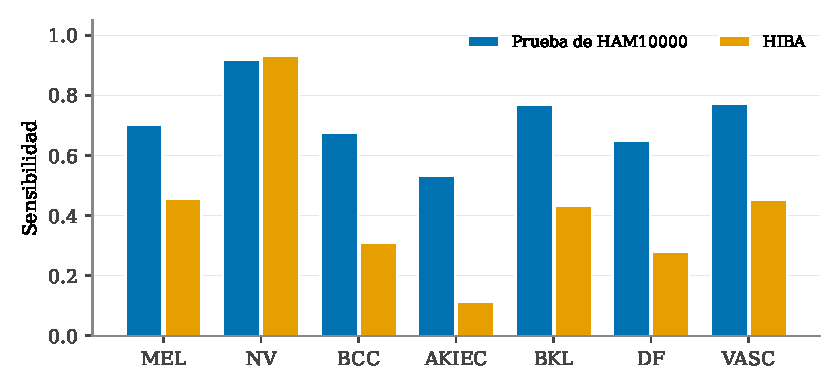
\includegraphics[width=0.85\textwidth]{Figures/Capitulos/04-Resultados-Clasificacion/hiba-por-clase-swin.pdf}
    \caption{Sensibilidad por clase de Swin-Tiny en la prueba de \emph{HAM10000} y en \emph{HIBA}.}
    \label{fig:res_hiba_clases}
\end{figure}

\subsection{Robustez a perturbaciones de la imagen}
\label{sec:res_robustez}

Sin cambiar de población, la segunda evaluación degrada las imágenes de la prueba con cuatro perturbaciones de
intensidad creciente. La Figura~\ref{fig:res_robustez} muestra la sensibilidad macro en cada nivel, y la
Tabla~\ref{tab:res_robustez}, la caída relativa (Ecuación~\ref{eq:marco_robustez}) en los niveles 1, 3 y 5. Como se
mide con una sola vista y sin \gls{tta}, la base es algo menor que la de la Tabla~\ref{tab:res_hiba}.

\begin{figure}[H]
    \centering
    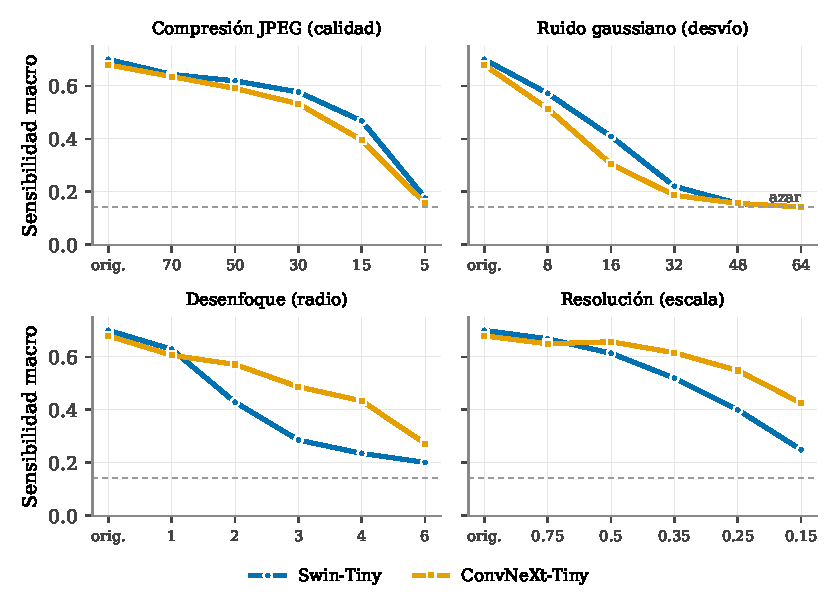
\includegraphics[width=0.85\textwidth]{Figures/Capitulos/04-Resultados-Clasificacion/robustez-curvas.pdf}
    \caption{Sensibilidad macro ante cuatro perturbaciones de intensidad creciente («orig.»: sin perturbar).}
    \label{fig:res_robustez}
\end{figure}

\begin{table}[H]
    \centering
    \caption{Caída relativa de la sensibilidad macro ante cuatro perturbaciones, por nivel de intensidad.}
    \label{tab:res_robustez}
    \small
    \setlength{\tabcolsep}{3pt}
    \begin{tabularx}{\textwidth}{@{}>{\raggedright\arraybackslash}X
        >{\centering\arraybackslash}p{1.1cm}>{\centering\arraybackslash}p{1.1cm}>{\centering\arraybackslash}p{1.1cm}
        >{\centering\arraybackslash}p{1.1cm}>{\centering\arraybackslash}p{1.1cm}>{\centering\arraybackslash}p{1.1cm}@{}}
        \toprule
        & \multicolumn{3}{c}{\textbf{Swin-Tiny}} & \multicolumn{3}{c}{\textbf{ConvNeXt-Tiny}} \\
        \cmidrule(lr){2-4}\cmidrule(l){5-7}
        \textbf{Perturbación (niveles 1, 3 y 5)} & \textbf{1} & \textbf{3} & \textbf{5} & \textbf{1} & \textbf{3}
            & \textbf{5} \\
        \midrule
        Compresión JPEG (calidad 70, 30 y 5) & 0.081 & 0.176 & 0.748 & 0.065 & 0.217 & 0.769 \\
        Ruido gaussiano (desvío 8, 32 y 64) & 0.184 & 0.685 & 0.796 & 0.244 & 0.725 & 0.790 \\
        Desenfoque (radio 1, 3 y 6) & 0.102 & 0.592 & 0.713 & 0.108 & 0.284 & 0.599 \\
        Resolución (0.75, 0.35 y 0.15) & 0.046 & 0.258 & 0.644 & 0.044 & 0.094 & 0.374 \\
        \bottomrule
    \end{tabularx}
\end{table}

Las degradaciones leves cuestan poco, salvo el ruido gaussiano, que es la perturbación más dañina: con un desvío de 8
sobre 255 ya quita casi un quinto de la sensibilidad macro, y en los niveles más altos lleva a los dos modelos al azar.
La compresión, en cambio, solo pesa cuando la calidad es muy baja. La diferencia más clara entre los dos modelos está
en el desenfoque y la reducción de resolución intensos, que ConvNeXt-Tiny soporta mejor. Estas perturbaciones
reproducen solo una parte de la variación real entre equipos (Sección~\ref{sec:marco_eval_robustez}), así que no
reemplazan la evaluación en \emph{HIBA}.

\subsection{Calibración}
\label{sec:res_calibracion}

Además de acertar la clase, el clasificador entrega probabilidades que fijan el umbral de melanoma y que un clínico
leería como certeza, y la tercera evaluación mide cuánto se puede confiar en ellas. La
Figura~\ref{fig:res_calibracion} muestra el diagrama de confiabilidad de Swin-Tiny con y sin pesos por clase, y la
Tabla~\ref{tab:res_calibracion} reúne el \gls{ece} y el Brier, también con los dos ajustes posteriores.

\begin{figure}[H]
    \centering
    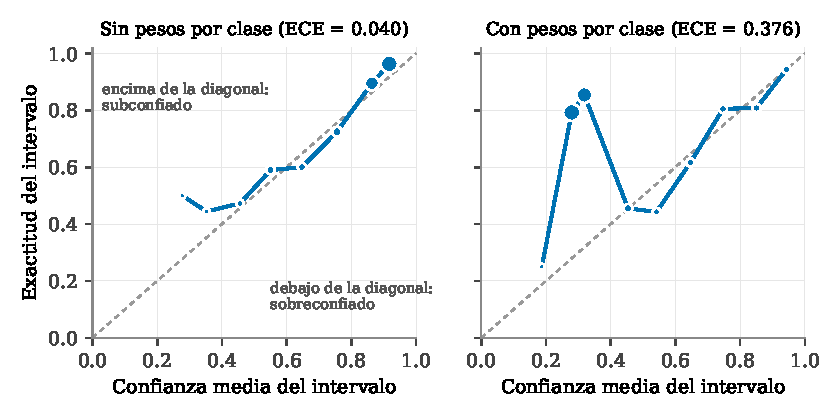
\includegraphics[width=0.85\textwidth]{Figures/Capitulos/04-Resultados-Clasificacion/calibracion-swin.pdf}
    \caption{Diagrama de confiabilidad de Swin-Tiny (semilla 42); el tamaño del punto es proporcional a la cantidad de imágenes del intervalo.}
    \label{fig:res_calibracion}
\end{figure}

\begin{table}[H]
    \centering
    \caption{Calibración en la prueba de \emph{HAM10000} (semilla 42). La fila con pesos por clase es la mejor configuración del barrido con pesos, distinta de la entropía cruzada ponderada de la Tabla~\ref{tab:res_desbalance}, que usa hiperparámetros fijos.}
    \label{tab:res_calibracion}
    \small
    \setlength{\tabcolsep}{4pt}
    \begin{tabularx}{\textwidth}{@{}>{\raggedright\arraybackslash}X
        >{\centering\arraybackslash}p{1.2cm}>{\centering\arraybackslash}p{1.2cm}>{\centering\arraybackslash}p{2.1cm}
        >{\centering\arraybackslash}p{1.2cm}>{\centering\arraybackslash}p{1.2cm}>{\centering\arraybackslash}p{2.1cm}@{}}
        \toprule
        & \multicolumn{3}{c}{\textbf{Swin-Tiny}} & \multicolumn{3}{c}{\textbf{ConvNeXt-Tiny}} \\
        \cmidrule(lr){2-4}\cmidrule(l){5-7}
        \textbf{Versión} & \textbf{ECE} & \textbf{Brier} & \textbf{Sensibilidad macro} & \textbf{ECE} & \textbf{Brier}
            & \textbf{Sensibilidad macro} \\
        \midrule
        Sin calibrar & 0.040 & 0.233 & 0.716 & 0.040 & 0.231 & 0.694 \\
        \emph{Temperature scaling} & 0.027 & 0.234 & 0.716 & 0.027 & 0.231 & 0.694 \\
        \emph{Vector scaling} & 0.014 & 0.216 & 0.675 & 0.033 & 0.226 & 0.687 \\
        \filasep
        Con pesos por clase & 0.376 & 0.609 & 0.770 & 0.211 & 0.636 & 0.742 \\
        \bottomrule
    \end{tabularx}
\end{table}

Sin pesos por clase, la curva sigue de cerca la diagonal, apenas por encima: el modelo es levemente subconfiado, es
decir, acierta algo más de lo que su confianza indica. Por eso la temperatura que ajusta la validación es menor que
uno, y con ella el \gls{ece} baja sin que cambie ninguna predicción. El vector scaling lo baja todavía más, pero
ajusta un parámetro por clase, cambia predicciones y reduce la sensibilidad macro. Con pesos por clase, en cambio, la
calibración se desarma: la confianza media cae a alrededor de 0.4 mientras la exactitud se mantiene cerca de 0.78, y
el \gls{ece} crece casi diez veces. En consecuencia, las probabilidades del modelo sin pesos pueden usarse casi sin
corrección, y las del modelo con pesos no deben leerse como certezas.

\subsection{Interpretabilidad}
\label{sec:res_interpretabilidad}

La última evaluación examina en qué parte de la imagen se apoya Swin-Tiny para decidir. La
Figura~\ref{fig:res_gradcam} muestra el mapa de Grad-CAM de la primera imagen de cada clase en la prueba. En las cinco
imágenes que el modelo clasifica bien (\gls{bkl}, \gls{df}, \gls{mel}, \gls{nv} y \gls{akiec}), la activación se
concentra sobre la lesión. De los dos errores, el \gls{bcc} clasificado como \gls{mel} también activa la lesión, lo
que sugiere una confusión entre lesiones pigmentadas y no una decisión tomada sobre el fondo. El \gls{vasc}
clasificado como \gls{nv}, en cambio, tiene una activación difusa sobre la piel que rodea la lesión. Como se trata de
siete imágenes, la inspección muestra que el modelo puede apoyarse en la lesión, pero no mide con qué frecuencia lo
hace ni prueba un razonamiento clínico (Sección~\ref{sec:met_interpretabilidad}).

\begin{figure}[H]
    \centering
    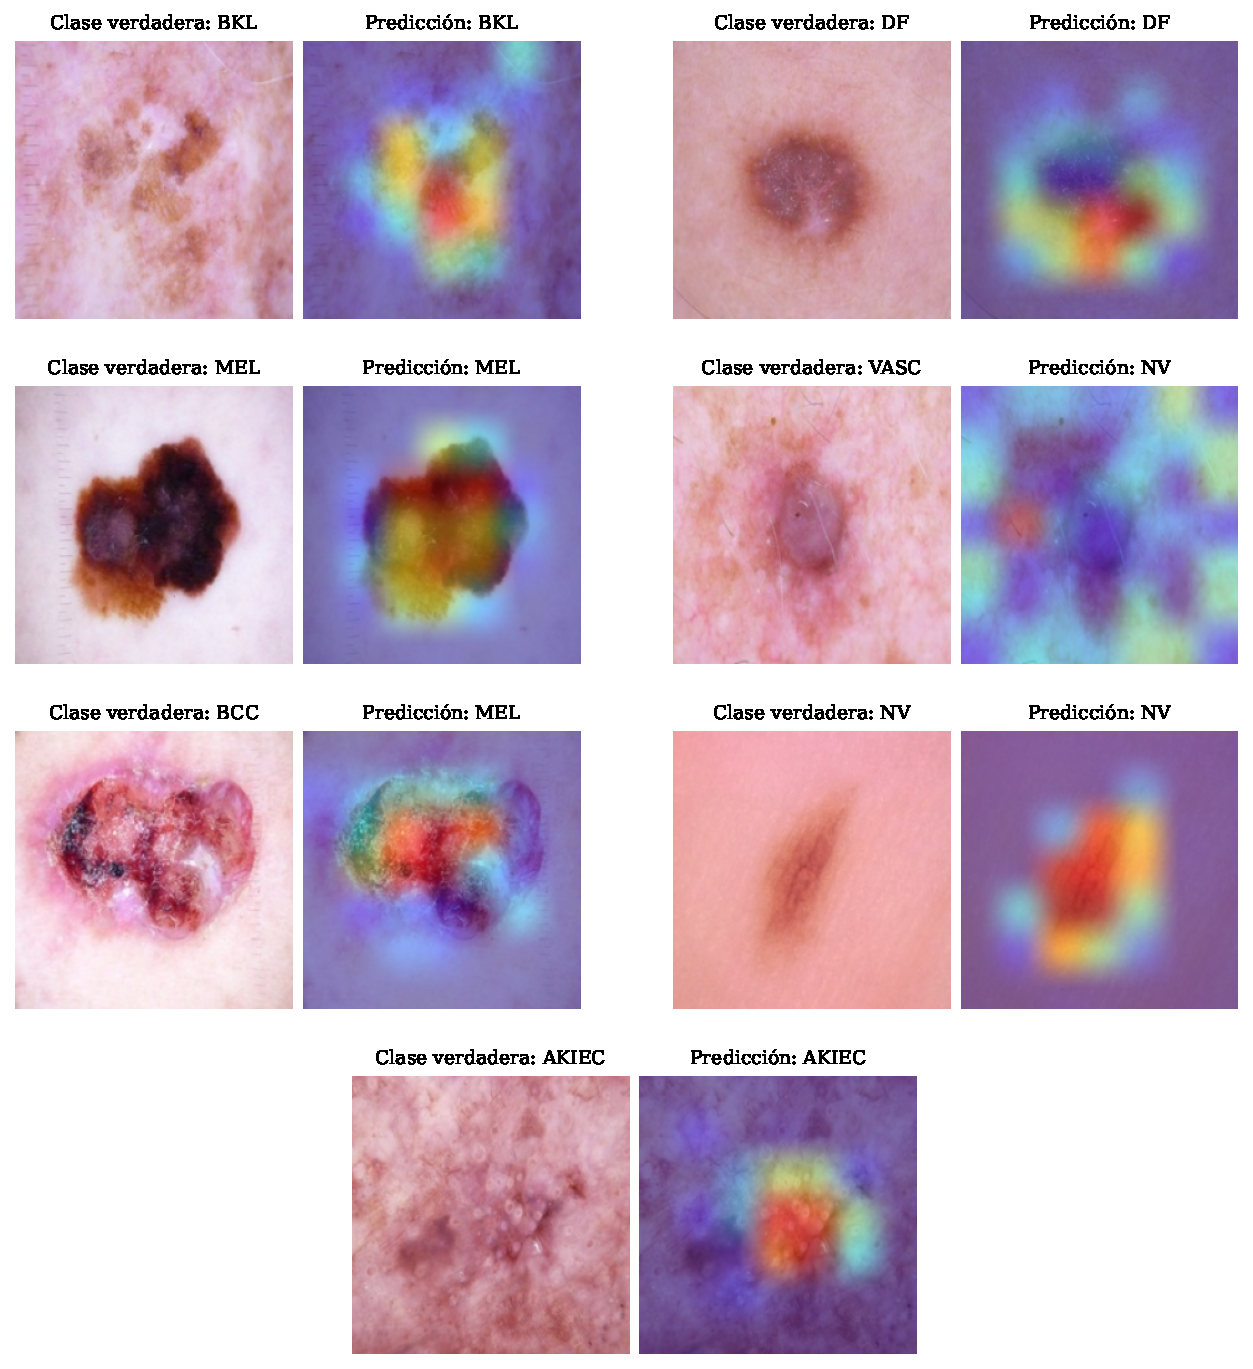
\includegraphics[width=0.9\textwidth]{Figures/Capitulos/04-Resultados-Clasificacion/gradcam-swin.pdf}
    \caption{Grad-CAM de Swin-Tiny sobre la primera imagen de prueba de cada clase.}
    \label{fig:res_gradcam}
\end{figure}

Con estas cuatro evaluaciones, el clasificador queda caracterizado también fuera de las condiciones de su
entrenamiento: pierde buena parte de su desempeño en otra población, es sensible al ruido de la imagen y entrega
probabilidades bien calibradas cuando se entrena sin pesos. Queda por ver si un \gls{vlm} podría ocupar su lugar, que es
lo que evalúa la sección siguiente.

\section{Clasificación con modelos visión--lenguaje}
\label{sec:res_vlm}
% Mini-VLM ajustado: checkpoint de generación v2, la configuración principal de la Sección 3.5 (LoRA solo en el
% codificador visual). La clasificación de la variante de control v3 no se usa (decisión del autor del 24/10/2026).
\pendiente{VLM generativos con las cuatro estrategias y el colapso; controles con imagen gris y con fotografías
clínicas; DermLIP con sus cuatro usos y el control con Swin-ImageNet; McNemar con Holm sobre los 21 pares; comparación
con la literatura.}

% Extensión estimada: unas 3 páginas, una subsección, dos tablas y una figura (ficha 4.4).
% Fuentes: ficha fichas/04-resultados-clasificacion/04-comparacion-modelos.md; Codigo/outputs/results/
% statistical_tests_les_v3.json (DermLIP con el protocolo oficial; v2 tenía el anterior), densenet_vit_moderna_report.json
% (holm, calculado sobre v2: los pares con DermLIP siguen con p < 1e-19 en v3), cost/cost_comparison_v3.json.
% Conteos de McNemar contra DermLIP (250/85, 286/89) recalculados de las predicciones de la semilla 42 y de
% dermlip/dermlip_zeroshot_vit-b-16_oficial_predictions.json.
% Figura: scripts/figuras_cap4.py (resumen-sensibilidad-macro.pdf).
% El label del costo es sec:res_costo_clasificadores: sec:res_costo es del Capítulo 5.
\section{Comparación entre los clasificadores y costo}
\label{sec:res_comparacion}

Las secciones anteriores evaluaron cada familia por separado. La Figura~\ref{fig:res_resumen} las reúne en una sola
escala, la sensibilidad macro en la prueba, y muestra tres niveles bien separados. Los supervisados quedan entre 0.6
y 0.7, con una variación pequeña entre semillas. DermLIP va desde algo más de 0.5 sin ajuste hasta el nivel de los supervisados
cuando se le entrena una cabeza. Los generativos, con cualquiera de sus cinco estrategias, quedan alrededor del azar.

\begin{figure}[H]
    \centering
    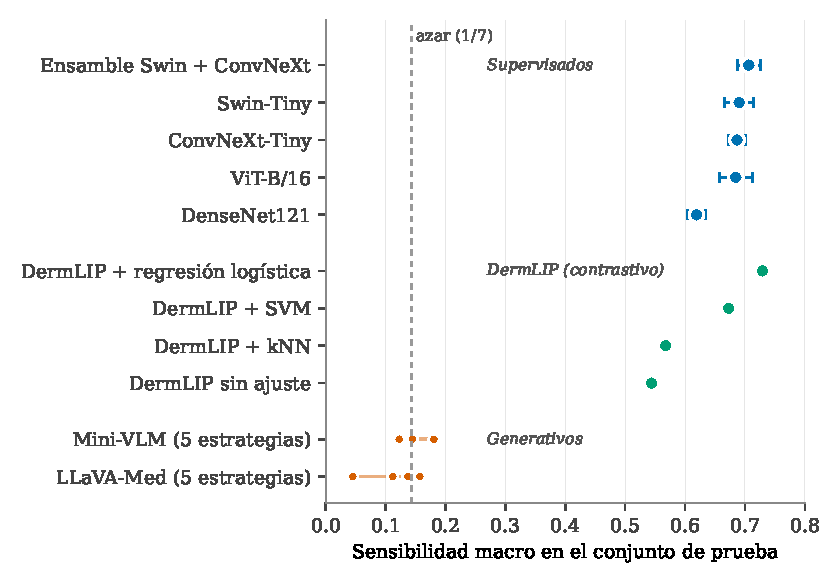
\includegraphics[width=0.85\textwidth]{Figures/Capitulos/04-Resultados-Clasificacion/resumen-sensibilidad-macro.pdf}
    \caption{Sensibilidad macro en la prueba de todos los clasificadores del capítulo. Los supervisados, con media y desvío de tres semillas; cada punto de los generativos es una estrategia.}
    \label{fig:res_resumen}
\end{figure}

Las pruebas de la Sección~\ref{sec:met_estadistica} confirman esa separación para los modelos sin ajuste, que entran
con la estrategia de generación en el caso de los generativos. En McNemar, los 15 pares de la familia de 21 que
comparan un supervisado con DermLIP, Mini-VLM o LLaVA-Med, o a estos tres entre sí, son significativos con la
corrección de Holm. La Tabla~\ref{tab:res_pruebas_vlm} muestra el tamaño de las diferencias en sensibilidad macro:
Swin-Tiny, ConvNeXt-Tiny y ViT-B/16 superan a DermLIP sin ajuste por entre 0.15 y 0.17, y a los generativos, por
alrededor de 0.5.

La única excepción es DenseNet121 frente a DermLIP. Su diferencia de sensibilidad macro no se distingue de cero, aunque
McNemar muestra que acierta más imágenes: DenseNet121 acierta 250 imágenes en las que DermLIP falla, frente a 85 en el
sentido contrario. Como en la comparación entre supervisados, la diferencia está en las clases mayoritarias, que pesan
mucho en el total de aciertos y poco en las métricas macro.

Entre los generativos, el intervalo de bootstrap de la sensibilidad macro de Mini-VLM incluye 1/7, de modo que
no se distingue del azar. El de LLaVA-Med queda apenas por encima, aunque su exactitud y su F1 macro siguen siendo
los de un modelo colapsado (Sección~\ref{sec:res_vlm}). Entre ellos, McNemar detecta que no aciertan las mismas
imágenes, pero la diferencia de sensibilidad macro no se distingue de cero, porque los dos aciertan pocas imágenes y
casi solo de la clase hacia la que colapsan.

\begin{table}[H]
    \centering
    \caption{Diferencia de sensibilidad macro entre cada supervisado y cada \gls{vlm} sin ajuste (semilla 42), con su IC del 95\,\%.}
    \label{tab:res_pruebas_vlm}
    \small
    \setlength{\tabcolsep}{4pt}
    \begin{tabularx}{\textwidth}{@{}>{\raggedright\arraybackslash}X ccc@{}}
        \toprule
        \textbf{Supervisado} & \textbf{DermLIP} & \textbf{Mini-VLM} & \textbf{LLaVA-Med} \\
        \midrule
        Swin-Tiny & 0.172 [0.116, 0.233] & 0.572 [0.522, 0.622] & 0.560 [0.510, 0.610] \\
        ConvNeXt-Tiny & 0.150 [0.092, 0.211] & 0.550 [0.501, 0.600] & 0.538 [0.488, 0.590] \\
        ViT-B/16 & 0.154 [0.105, 0.209] & 0.554 [0.503, 0.606] & 0.542 [0.490, 0.595] \\
        DenseNet121 & 0.050 [$-$0.016, 0.120] & 0.450 [0.398, 0.508] & 0.438 [0.385, 0.495] \\
        \bottomrule
    \end{tabularx}
\end{table}

La comparación deja abierta la posición de DermLIP con una cabeza entrenada, que se acerca a los supervisados en
sensibilidad macro pero no en F1 macro (Tabla~\ref{tab:res_dermlip}). Como esa cabeza se entrena sobre
\emph{HAM10000}, deja de ser un uso sin ajuste y no resuelve lo que motivaba usar un \gls{vlm}: obtener el diagnóstico
del modelo que genera el reporte.

\subsection{Costo computacional de los clasificadores}
\label{sec:res_costo_clasificadores}

Además del desempeño, la restricción de una GPU de consumo de la Sección~\ref{sec:met_tareas} exige que el
clasificador sea barato de ejecutar. La Tabla~\ref{tab:res_costo_clasificadores} reúne su costo en la RTX 4070 de la
Sección~\ref{sec:met_entorno}, con la misma precisión bf16 que la evaluación. Los cuatro modelos clasifican una
imagen en 20~ms o menos y ocupan menos de 0.7~GB de memoria de la GPU aun con lotes de 32 imágenes. Con esos lotes,
Swin-Tiny clasifica la prueba completa en poco más de un segundo, y con una imagen por vez, en unos 17 segundos.
Además, la cantidad de parámetros no ordena el tiempo de inferencia: DenseNet121, el modelo más chico, es el más lento
con una imagen por vez. Estos tiempos corresponden a una sola vista, y el \gls{tta} de la
Sección~\ref{sec:met_supervisados_receta} duplica las pasadas. Aun así, el costo de los clasificadores queda muy por
debajo de ese límite.

\begin{table}[H]
    \centering
    \caption{Costo de inferencia de los clasificadores en una RTX 4070 (bf16, una vista por imagen). La latencia se mide con una imagen por vez, y las imágenes por segundo, con lotes de 32.}
    \label{tab:res_costo_clasificadores}
    \small
    \setlength{\tabcolsep}{3pt}
    \begin{tabularx}{\textwidth}{@{}>{\raggedright\arraybackslash}X
        >{\centering\arraybackslash}p{1.9cm}>{\centering\arraybackslash}p{2.0cm}>{\centering\arraybackslash}p{2.0cm}
        >{\centering\arraybackslash}p{1.9cm}>{\centering\arraybackslash}p{2.0cm}@{}}
        \toprule
        & & \multicolumn{2}{c}{\textbf{Memoria máxima (GB)}} & & \\
        \cmidrule(lr){3-4}
        \textbf{Modelo} & \textbf{Parámetros (millones)} & \textbf{Una imagen} & \textbf{Lote de 32}
            & \textbf{Latencia (ms)} & \textbf{Imágenes por segundo} \\
        \midrule
        Swin-Tiny & 27.52 & 0.180 & 0.522 & 11.05 & 1\,353.3 \\
        ConvNeXt-Tiny & 27.83 & 0.179 & 0.407 & 4.99 & 1\,738.5 \\
        ViT-B/16 & 85.80 & 0.511 & 0.678 & 5.72 & 903.5 \\
        DenseNet121 & 6.96 & 0.052 & 0.216 & 19.89 & 1\,700.3 \\
        \bottomrule
    \end{tabularx}
\end{table}

Con el desempeño y el costo de las tres familias caracterizados, queda ubicar estos resultados frente a los de la
literatura.

% Extensión estimada: unas 2.5 páginas, cuatro párrafos y una tabla (ficha 4.5).
% Fuentes: Tablas tab:marco_sota_clasificacion, tab:marco_sota_vlm y tab:marco_sota_vlm_gen del Capítulo 2 y las
% cifras de las secciones 4.1 a 4.4. Reúne las comparaciones con la literatura que antes estaban repartidas en cada
% sección (revisión del autor, 24/10/2026).
\section{Comparación con el estado del arte}
\label{sec:res_estado_arte}

Los trabajos del Capítulo~\ref{cp:marco} no permiten una comparación directa con estos resultados, porque difieren en
los datos, en la forma de dividirlos y en la regla de decisión. Por eso, esta sección no ordena los modelos, sino que
ubica el orden de magnitud de los resultados y examina qué parte de las diferencias se explica por el protocolo. La
Tabla~\ref{tab:res_estado_arte} reúne las cifras comparables en tres bloques: la clasificación en siete clases, la
detección de melanoma y los \glspl{vlm} sin ajuste. Cada fila es un trabajo, con sus datos y su protocolo, la métrica
que se compara, el valor que informa y el del modelo equivalente de este trabajo.

\begin{table}[H]
    \centering
    \caption{Resultados de la literatura (Capítulo~\ref{cp:marco}) frente a los de este trabajo. «---»: sin cifra equivalente.}
    \label{tab:res_estado_arte}
    \footnotesize
    \setlength{\tabcolsep}{3pt}
    \begin{tabularx}{\textwidth}{@{}>{\raggedright\arraybackslash}p{2.6cm}
        >{\raggedright\arraybackslash\hspace{0pt}}X
        >{\raggedright\arraybackslash\hspace{0pt}}p{2.5cm}
        >{\centering\arraybackslash}p{1.9cm}>{\centering\arraybackslash}p{1.9cm}@{}}
        \toprule
        \textbf{Trabajo} & \textbf{Datos y protocolo} & \textbf{Métrica} & \textbf{Trabajo citado}
            & \textbf{Este trabajo} \\
        \midrule
        \multicolumn{5}{@{}l}{\textit{Clasificación en siete clases (Swin-Tiny)}} \\
        \textcite{aboulmira2024skinhealthmate} & \emph{HAM10000}; partición no informada & F1 macro & 0.81 & 0.733 \\
        \textcite{kim2025skinsavvy2} & \emph{HAM10000} ampliado; partición al azar por imagen & Sensibilidad macro
            & 0.780 & 0.692 \\
        \textcite{gessert2020skin} & \emph{ISIC 2019}, otras clases; prueba del desafío; validación por lesión & Sensibilidad macro & 0.636
            & 0.692 \\
        \filasep
        \multicolumn{5}{@{}l}{\textit{Detección de melanoma (Swin-Tiny)}} \\
        \textcite{aboulmira2024skinhealthmate} & Clase más probable & Sensibilidad & 0.49 & 0.623 \\
        \textcite{yao2022single} & \emph{ISIC 2018}; modelo elegido sobre la prueba & Sensibilidad & 0.819 & 0.796 \\
        \textcite{marchetti2023prospective} & Lesiones biopsiadas; umbral de alta sensibilidad & AUC & 0.857
            & 0.921 \\
        \filasep
        \multicolumn{5}{@{}l}{\textit{\glspl{vlm} sin ajuste}} \\
        \textcite{yan2025derm1miccv} & DermLIP en \emph{HAM10000} & Exactitud & 0.682 & 0.716 \\
        \textcite{yan2026dermfmzero} & DermFM-Zero en siete conjuntos; DermLIP obtiene 0.561 & Exactitud balanceada y AUC, en media
            & 0.733 & --- \\
        \textcite{zeng2025mmskin} & LLaVA-Med en \emph{HAM10000} & Exactitud & 0.055 & 0.037--0.114 \\
        \textcite{zeng2025mmskin} & SkinVL, especializado, en \emph{HAM10000} & Exactitud & 0.513 & --- \\
        \textcite{jiang2026multimodal} & Generativos abiertos en consultas reales; tres primeros diagnósticos
            & Exactitud & 0.015--0.134 & --- \\
        \bottomrule
    \end{tabularx}
\end{table}

En la clasificación de siete clases, los resultados de Swin-Tiny quedan por debajo de los dos trabajos que usan
\emph{HAM10000}, pero ninguno de ellos divide las imágenes por lesión: uno no informa cómo las divide, y el otro amplía
el conjunto con imágenes externas y lo divide al azar por imagen. La Sección~\ref{sec:res_fuga} mostró que, en esta
prueba, una partición por imagen sobreestima la sensibilidad macro en unas 0.07, una cifra del mismo orden que la
distancia con el segundo trabajo. Por el contrario, el único trabajo que mantiene juntas las imágenes de una lesión
informa una sensibilidad macro algo menor que la de Swin-Tiny, aunque sobre otro conjunto y con otras clases. La
comparación no permite atribuir toda la distancia a la partición, porque los trabajos difieren también en los datos y
en el entrenamiento, pero sí muestra que una parte puede deberse a ella.

En la detección de melanoma, la tabla muestra que la sensibilidad depende tanto de la regla de decisión como del
modelo. Con la clase más probable, Swin-Tiny detecta más melanomas que el ensamble de
\textcite{aboulmira2024skinhealthmate}, que usa la misma regla. El trabajo de \textcite{yao2022single} obtiene una
sensibilidad algo mayor que la de Swin-Tiny con el umbral de validación, pero elige su modelo sobre la misma prueba
en que lo informa. En el otro extremo, \textcite{marchetti2023prospective} operan con una sensibilidad cercana a la
total a cambio de una especificidad baja, sobre lesiones que ya habían sido biopsiadas. Como cada trabajo usa otra
población y otro punto de operación, la comparación no ordena los modelos, pero justifica que este trabajo fije el
umbral en validación y lo informe junto con la sensibilidad.

En los \glspl{vlm} generativos, los resultados coinciden con la literatura. \textcite{zeng2025mmskin} miden LLaVA-Med
sin ajuste en \emph{HAM10000} con una exactitud del 5.5\,\%, dentro del rango que obtiene aquí, y solo su modelo
especializado, SkinVL, supera el 50\,\%. Del mismo modo, \textcite{jiang2026multimodal} informan exactitudes de entre el 1.5\,\% y el 13.4\,\% con los modelos abiertos en
consultas reales, entre ellos LLaVA-Med. Por lo tanto, el colapso de los generativos de propósito general no es propio
de este trabajo. También DermLIP sin ajuste, con las plantillas y los nombres de clase de sus autores, obtiene en
\emph{HAM10000} una exactitud cercana a la que ellos informan, sobre otra partición de prueba. DermFM-Zero, evaluado
por sus autores junto con DermLIP, lo supera a su vez, lo que indica que la especialización en dermatología sigue
mejorando por la vía contrastiva.

En conjunto, la comparación ubica a Swin-Tiny cerca de los trabajos con un protocolo comparable y por debajo de los que
usan una partición por imagen, y confirma que la dificultad de los \glspl{vlm} generativos para clasificar lesiones de
piel aparece también en la literatura.

% Extensión estimada: una página, cuatro párrafos (ficha 4.6).
% Fuentes: secciones 4.1 a 4.5. Sin números nuevos.
% Feedback del tutor (14/09/2026): el cierre se llama "Discusión"; la discusión que cruza clasificación y generación
% queda en el Capítulo 6.
\section{Discusión de los resultados de clasificación}
\label{sec:res_clasif_discusion}

Los resultados del capítulo permiten responder la primera pregunta de investigación
(Sección~\ref{sec:intro_objetivos}): en la prueba de \emph{HAM10000}, ningún \gls{vlm} sin una cabeza entrenada sobre
ese conjunto clasifica las lesiones tan bien como un clasificador supervisado. Los \glspl{vlm} generativos de propósito general quedan en el nivel del azar y
colapsan hacia una clase que depende del modelo y de la estrategia, y los controles muestran que ese comportamiento no
se explica por el desbalance de las clases ni por la modalidad de la imagen. DermLIP, en cambio, muestra que la
especialización en dermatología aporta una representación útil, pero solo se acerca a los supervisados con una cabeza
entrenada sobre \emph{HAM10000}. Las diferencias con los modelos sin ajuste son, además, significativas en McNemar,
salvo la de DenseNet frente a DermLIP en sensibilidad macro, y coinciden con lo que informa la literatura.

Entre los clasificadores supervisados, en cambio, la arquitectura pesa menos que otros factores. Con el mismo
procedimiento, Swin-Tiny, ConvNeXt-Tiny y ViT-B/16 no se distinguen entre sí, mientras que la semilla cambia la
sensibilidad de las clases minoritarias y del melanoma en más de una décima. En melanoma, la regla de decisión pesa más
que el modelo: el umbral fijado en validación lleva la detección de tres a cuatro de cada cinco casos sin cambiar el
\gls{auc}. Del mismo modo, la partición cambia el resultado, ya que una partición por imagen sobreestima la
sensibilidad macro en unas 0.07. Por ello, una comparación con otros trabajos tiene sentido solo cuando se conocen
su partición y su regla de decisión.

Estos resultados valen dentro de la fuente de entrenamiento. En \emph{HIBA}, Swin-Tiny pierde cerca del 40\,\% de su
sensibilidad macro, también en las imágenes dermatoscópicas, y el ruido de la imagen lo afecta más que la compresión
o la pérdida de resolución. Sus probabilidades, en cambio, están bien calibradas cuando se entrena sin pesos por clase.
En consecuencia, Swin-Tiny es la referencia del trabajo dentro de \emph{HAM10000}, pero no una herramienta validada
para otra población, y las limitaciones que eso implica, junto con las de evaluar las pruebas con una sola semilla, se
retoman en el Capítulo~\ref{cp:discusion}.

Estos resultados determinan también de dónde sale el diagnóstico del \emph{pipeline}. Como un \gls{vlm} generativo no
distingue las siete clases, el diagnóstico no puede salir del generador, y por eso lo fija Swin-Tiny, que se lo
entrega al generador a través de la cascada (Sección~\ref{sec:met_cascada}). Como el clasificador ocupa menos de
1~GB de memoria y clasifica una imagen en milisegundos, el costo del pipeline lo fija el generador. El
Capítulo~\ref{cp:res_gen} evalúa si, con ese diagnóstico, el reporte generado afirma la clase correcta y cuánto cuesta
generarlo, y la discusión que cruza ambos resultados queda para el Capítulo~\ref{cp:discusion}.

